%% ===========================================================================
%%  Large Language Models for Software Requirements Classification:
%%  Cross-Dataset Generalisation and Cost-Efficiency
%%
%%  IEEE conference format (ICCI 2026), 8 pages.
%%  Every number quoted below is written by scripts/make_numbers.py, which
%%  reads it out of the stored pipeline artefacts; the tables in tables/ and
%%  the figures in figures/ come from the same artefacts.  Nothing here is
%%  typed in by hand.
%% ===========================================================================
\documentclass[conference]{IEEEtran}
\IEEEoverridecommandlockouts

\usepackage{cite}
\usepackage{amsmath,amssymb}
\usepackage{graphicx}
\usepackage{booktabs}
\usepackage{xcolor}
\usepackage{microtype}
\usepackage{url}
\usepackage{tikz}
\usetikzlibrary{positioning,arrows.meta,fit,backgrounds,calc,shapes.geometric,
                decorations.pathreplacing,patterns}
\usepackage[hidelinks]{hyperref}
\usepackage{balance}
\usepackage{pifont}
\newcommand{\cmark}{\ding{51}}
\newcommand{\xmark}{\ding{55}}

\newcommand{\pex}{PROMISE\_exp}
\newcommand{\Fm}{macro-F1}
\definecolor{encblue}{HTML}{0072B2}
\definecolor{llmgold}{HTML}{E69F00}
\definecolor{panel}{HTML}{F2F4F7}
\definecolor{rule}{HTML}{9AA3AD}

%% Generated by scripts/make_numbers.py -- do not edit by hand.
\newcommand{\nAheadXP}{76}
\newcommand{\nBEmax}{552}
\newcommand{\nBEmed}{215}
\newcommand{\nBEmin}{46}
\newcommand{\nCostEnc}{0.0024}
\newcommand{\nCostLLMmax}{0.0704}
\newcommand{\nCostLLMmin}{0.0248}
\newcommand{\nDropXDBu}{41.1}
\newcommand{\nDropXDRu}{21.8}
\newcommand{\nDropXDRw}{22.7}
\newcommand{\nDropXDmax}{42.8}
\newcommand{\nDropXDmin}{15.5}
\newcommand{\nDropXDrevMax}{17.4}
\newcommand{\nDropXDrevMin}{15.5}
\newcommand{\nDropXPmax}{29.6}
\newcommand{\nDropXPpromMax}{11.9}
\newcommand{\nDropXPpromMin}{3.0}
\newcommand{\nFsBinMean}{$-$0.007}
\newcommand{\nFsBinN}{54}
\newcommand{\nFsMed}{+0.024}
\newcommand{\nFsSubMean}{+0.062}
\newcommand{\nFsSubN}{36}
\newcommand{\nGemmaSec}{0.900}
\newcommand{\nGpuOnDemand}{0.5260}
\newcommand{\nGpuSource}{AWS EC2 g4dn.xlarge (1x T4), us-east-1, verified 2026-08-06}
\newcommand{\nGpuSpot}{0.3162}
\newcommand{\nLLMnfrMax}{43.4}
\newcommand{\nLLMnfrMin}{14.9}
\newcommand{\nLLMnfrMinModel}{Qwen2.5-3B}
\newcommand{\nLatCom}{0.614}
\newcommand{\nLatEnc}{0.016}
\newcommand{\nLatHost}{0.095}
\newcommand{\nLatLocMax}{0.356}
\newcommand{\nLatLocMin}{0.194}
\newcommand{\nLeadAll}{0.095}
\newcommand{\nLeadFour}{0.014}
\newcommand{\nLeadFourCommon}{0.036}
\newcommand{\nLlamaSec}{0.891}
\newcommand{\nLossID}{0}
\newcommand{\nLossXD}{48}
\newcommand{\nLossXP}{14}
\newcommand{\nNBE}{276}
\newcommand{\nNGemini}{60}
\newcommand{\nNLLMprior}{8}
\newcommand{\nNPareto}{10}
\newcommand{\nNParetoEnc}{9}
\newcommand{\nNcellItems}{968/444/968/353/433/524}
\newcommand{\nNcells}{87}
\newcommand{\nNcellsdrop}{6}
\newcommand{\nNcellsrep}{81}
\newcommand{\nNcommonFour}{59}
\newcommand{\nNdup}{67}
\newcommand{\nNfolds}{107}
\newcommand{\nNfrPromise}{444}
\newcommand{\nNfsTests}{90}
\newcommand{\nNgroups}{50}
\newcommand{\nNlocalCfg}{10}
\newcommand{\nNnfrPromise}{524}
\newcommand{\nNppProj}{37}
\newcommand{\nNpred}{76,115}
\newcommand{\nNpredEnc}{24,280}
\newcommand{\nNpredLLM}{51,835}
\newcommand{\nNpromise}{968}
\newcommand{\nNpromiseProj}{47}
\newcommand{\nNpromiseRaw}{969}
\newcommand{\nNpromptMax}{960}
\newcommand{\nNpromptMin}{59}
\newcommand{\nNpsCells}{9}
\newcommand{\nNpsRows}{12,042}
\newcommand{\nNsecPromise}{125}
\newcommand{\nNsecSecreq}{177}
\newcommand{\nNsecreq}{444}
\newcommand{\nNsecreqProj}{3}
\newcommand{\nNsecreqRaw}{510}
\newcommand{\nNshared}{0}
\newcommand{\nNsplitfam}{14}
\newcommand{\nNsubtypeall}{524}
\newcommand{\nNsubtypefour}{353}
\newcommand{\nNsubtypesix}{433}
\newcommand{\nNtestGemini}{26}
\newcommand{\nNtestID}{106}
\newcommand{\nNtestXD}{64}
\newcommand{\nNtestXP}{90}
\newcommand{\nNtests}{260}
\newcommand{\nNtotal}{1,412}
\newcommand{\nOracleMax}{0.036}
\newcommand{\nOracleMed}{0.003}
\newcommand{\nParetoGain}{0.010}
\newcommand{\nParetoLLM}{Qwen2.5-7B}
\newcommand{\nParetoRatio}{19}
\newcommand{\nPpEncMed}{0.917}
\newcommand{\nPpEncSdMax}{0.198}
\newcommand{\nPpEncSdMin}{0.193}
\newcommand{\nPpLocMedMax}{0.750}
\newcommand{\nPpLocMedMin}{0.545}
\newcommand{\nPpLocSdMax}{0.301}
\newcommand{\nPpLocSdMin}{0.213}
\newcommand{\nPrecID}{0.847}
\newcommand{\nPrecXD}{0.210}
\newcommand{\nPrevPromise}{12.9}
\newcommand{\nPrevSecreq}{39.9}
\newcommand{\nPriceGemIn}{0.25}
\newcommand{\nPriceGemOut}{1.50}
\newcommand{\nPriceLlaIn}{0.59}
\newcommand{\nPriceLlaOut}{0.79}
\newcommand{\nPsParse}{99.83}
\newcommand{\nRatioMax}{29}
\newcommand{\nRatioMed}{19}
\newcommand{\nRatioMin}{10}
\newcommand{\nRecID}{0.888}
\newcommand{\nRecXD}{0.720}
\newcommand{\nRhoPrior}{0.95}
\newcommand{\nRhoSize}{0.85}
\newcommand{\nSecreqBestEnc}{0.836}
\newcommand{\nSecreqBestLLM}{0.846}
\newcommand{\nSecreqP}{0.696}
\newcommand{\nSecreqPBH}{0.774}
\newcommand{\nShareBertID}{13.5}
\newcommand{\nShareBertRev}{33.6}
\newcommand{\nShareBertXD}{44.2}
\newcommand{\nShareNFR}{54.1}
\newcommand{\nShareRobRev}{29.1}
\newcommand{\nShareRobXD}{19.7}
\newcommand{\nSigBH}{170}
\newcommand{\nSigHolm}{131}
\newcommand{\nSigRaw}{175}
\newcommand{\nSpreadMax}{0.485}
\newcommand{\nSpreadMed}{0.044}
\newcommand{\nTenkEnc}{0.03}
\newcommand{\nTenkGem}{0.25}
\newcommand{\nTenkLla}{0.70}
\newcommand{\nTenkQwen}{0.31}
\newcommand{\nTerseShare}{96.7}
\newcommand{\nTerseTrue}{39.7}
\newcommand{\nTieGemini}{23}
\newcommand{\nTieID}{39}
\newcommand{\nTieXD}{13}
\newcommand{\nTieXP}{38}
\newcommand{\nTrainMed}{0.0089}
\newcommand{\nTrainSec}{172}
\newcommand{\nWinID}{67}
\newcommand{\nWinXD}{3}
\newcommand{\nWinXP}{38}
\newcommand{\nXDrefF}{0.923}
\newcommand{\nXDtransF}{0.528}
     % every reported figure, generated from the artefacts

% pack floats a little more densely than the conservative defaults
\renewcommand{\topfraction}{0.92}
\renewcommand{\bottomfraction}{0.85}
\renewcommand{\textfraction}{0.06}
\renewcommand{\floatpagefraction}{0.75}
\setcounter{topnumber}{3}
\setcounter{bottomnumber}{2}
\setcounter{totalnumber}{4}

\begin{document}

\title{Large Language Models for Software Requirements\\Classification:
       Cross-Dataset Generalisation and Cost-Efficiency}

\author{\IEEEauthorblockN{Fatma El-Zahraa Samir, Khaled T. Wassif, and Lamia AbouZeid}
\IEEEauthorblockA{\textit{Faculty of Computers and Artificial Intelligence},
\textit{Cairo University}, Giza, Egypt\\
fatmaelzahraasamirabdelfattah@gmail.com}}

\maketitle

\begin{abstract}
Recent work reports that prompting a large language model (LLM) classifies
software requirements about as well as fine-tuning a small transformer, and that
labelled training data may therefore no longer be needed. Nearly all of that
evidence is collected in one place: the model is fitted, or its examples chosen,
on the corpus that also supplies the test items, and what the technique costs to
run is rarely reported. This paper repeats the comparison with both gaps closed.
Fine-tuned encoders and prompted LLMs from three access tiers classify the same
requirements from two public corpora, under the same tasks and the same scoring
rule, at three levels of distribution shift: inside one corpus, across held-out
projects, and across a corpus annotated by a different team. Every encoder--LLM
comparison is paired on identical items and corrected for multiple testing as a
single family. The ranking of the two approaches is not stable across those
levels: inside a corpus the encoders lead and are never significantly beaten,
but once the test corpus is annotated by someone else the ordering reverses. The
reason is not that the transferred encoder fails to recognise the new
vocabulary; it carries over the class balance of the corpus it was trained on,
so it goes on finding the rare class far too often. The prompted models have the
same weakness from a different source, since their class balance is set by the
wording of the instruction. The encoders nevertheless remain an order of
magnitude cheaper per item and repay their one-off training after a few hundred
classifications. The evaluation regime therefore belongs in the claim: a score
obtained in-distribution does not predict which approach wins once the corpus
changes, and can point the wrong way.
\end{abstract}

\begin{IEEEkeywords}
requirements classification, large language models, fine-tuning,
generalisation, distribution shift, empirical software engineering,
cost-efficiency
\end{IEEEkeywords}

%% ===========================================================================
\section{Introduction}
%% ===========================================================================
Requirements classification assigns a natural-language requirement statement to
a category, such as functional (FR) against non-functional (NFR), or
security-relevant against not. ISO/IEC/IEEE 29148 defines requirements and their
attributes across the life cycle~\cite{iso29148}, and classification is one of
the first analytical steps after elicitation. Doing it well supports early risk
identification and architectural choice; doing it badly propagates downstream as
rework~\cite{clelandhuang2007}. Two decades of automation moved the task from
weighted indicator terms~\cite{clelandhuang2007} through supervised learning on
engineered features~\cite{kurtanovic2017} to fine-tuned
transformers~\cite{hey2020norbert}, and since 2024 to prompted generative
LLMs~\cite{elhajjami2024,binkhonain2025,alhoshan2025,tang2025,levy2026}; the
systematic mapping of Kaur and Kaur documents the same
progression~\cite{kaur2024}.

It is worth being precise about what that literature claims, because the
motivation for this study is often summarised too strongly. We are not aware of
any paper stating that requirements classification is solved. What several
report is parity or better between prompting and supervision on the corpora they
use: Binkhonain and Alfayaz find that few-shot prompting matches or exceeds a
fine-tuned transformer and conclude that prompting is viable where labelled data
is scarce~\cite{binkhonain2025}; Tang et al.\ report an 8\,B open model passing a
fine-tuned baseline on PROMISE~\cite{tang2025}; and Alhoshan et al.\ report that
generative models perform competitively without task-specific
training~\cite{alhoshan2025}, extending earlier evidence that zero-shot embedding
methods had already made labelled data non-essential~\cite{alhoshan2023}.
Together these make ``prompting can replace fine-tuning'' a reasonable reading of
the state of the art, and it is that reading, rather than any individual paper's
claim, that this study puts to the test.

The reading rests on a measurement convention. Almost every published result is
obtained in-distribution: the model is fine-tuned, or its exemplars selected, on
the corpus that then supplies the test items. Where prior work reports improved
generalisability it usually means transfer across \emph{tasks} on the same
corpora rather than to unseen projects or an independent
dataset~\cite{binkhonain2025} --- the weakness NoRBERT was built to address,
since it was motivated by classifiers over-fitting project-specific
wording~\cite{hey2020norbert}. A second omission compounds the first: inference
cost, latency and model size are seldom quantified, although they decide whether
a technique can be adopted at all without a commercial API budget.

This paper asks what happens when both omissions are repaired. We hold the
corpus, the items, the label sets and the scoring rule fixed, and vary only the
distance between the data a model was fitted on and the data it is scored on. We
contribute a paired, multiplicity-controlled benchmark of twelve configurations
over three tasks, two corpora and three regimes; evidence that the ranking
depends on the regime; a diagnosis of the cause as a mis-set class prior that
both families share; and an accuracy--cost comparison priced from the runs
themselves. \textbf{RQ1}: how do open and commercial LLMs compare with fine-tuned
encoders within one corpus? \textbf{RQ2}: how much is lost under cross-project
and cross-dataset evaluation, and does the loss differ between the families?
\textbf{RQ3}: what is the accuracy-versus-cost trade-off, and what is the
cheapest freely available option that is good enough?

%% ===========================================================================
\section{Related Work and the Evaluation Gap}
%% ===========================================================================
\subsection{From indicator terms to prompting}
Rule-based work established the task and produced the PROMISE NFR
collection~\cite{clelandhuang2007}; classical supervised learning followed, with
SVMs separating FRs from NFRs~\cite{kurtanovic2017}. Transfer learning then reset
the state of the art: NoRBERT fine-tunes BERT and reports \Fm{} in the mid
nineties on the PROMISE categories~\cite{hey2020norbert}, a pattern the
systematic mapping of Kaur and Kaur later confirmed~\cite{kaur2024}. Zero-shot
embedding methods showed labelled data was not strictly
necessary~\cite{alhoshan2023}, and prompted generative LLMs now dominate.

\subsection{Recent LLM studies, 2024--2026}
Binkhonain and Alfayaz~\cite{binkhonain2025} report the study closest to ours:
five LLMs under four prompting strategies over three tasks on PROMISE and
SecReq, against a fine-tuned transformer that few-shot prompting matches or
exceeds. Alhoshan et al.~\cite{alhoshan2025} ran more than 400 experiments over
three open generative models, and Tang et al.~\cite{tang2025} identified an
over-prompting effect in which extra in-context examples degrade accuracy.
Elsewhere the task has been compared across classical and generative
techniques~\cite{elhajjami2024}, embedded in a systems engineering
workflow~\cite{peer2024}, extended to app-store reviews~\cite{chaudhary2025},
run against GPT-4o~\cite{vasudevan2026} and benchmarked against expert
judgment~\cite{levy2026}.

\subsection{What this literature does not measure}
Table~\ref{tab:coverage} summarises the evaluation coverage of those studies
along the axes that decide whether a result transfers to practice, and three
patterns recur. First, evaluation is in-distribution: the same corpus supplies
the training data or the exemplars and the test items. Only the app-review
study~\cite{chaudhary2025} tests genuinely different text, and it reports
markedly lower precision on several categories, a signal the literature has not
followed up. Second, cost is not reported, even in the studies that use open
models~\cite{alhoshan2025,tang2025}. Third, the same few small, ageing, public
corpora underlie nearly every result, so contamination of LLM pre-training data
is acknowledged but not addressed~\cite{sainz2023}. These gaps interact: if
in-distribution parity is what motivates replacing supervision with prompting,
and is also what corpus reuse and contamination would produce spuriously, then
the comparison that settles the question has not yet been run.

\begin{table}[t]
\caption{Evaluation coverage of recent LLM-based requirements-classification
studies. \cmark{} = reported; \xmark{} = not reported; $\sim$ = partially.
``Cross-project'' means held-out unseen projects; ``cross-dataset'' means an
independently produced corpus. The table describes prior work only.}
\label{tab:coverage}
\centering
\scriptsize
\setlength{\tabcolsep}{3.6pt}
\renewcommand{\arraystretch}{1.03}
\begin{tabular}{@{}lccccc@{}}
\toprule
& \textbf{Open} & \textbf{Comm.} & \textbf{Cross-} & \textbf{Cross-} & \textbf{Cost} \\
\textbf{Study} & LLMs & LLMs & project & dataset & \\
\midrule
El-Hajjami et al.~\cite{elhajjami2024}   & \xmark & \cmark & \xmark & \xmark & \xmark \\
Peer et al.~\cite{peer2024}              & \xmark & \cmark & \xmark & \xmark & $\sim$ \\
Binkhonain \& Alfayaz~\cite{binkhonain2025} & \cmark & \cmark & \xmark & \xmark & \xmark \\
Alhoshan et al.~\cite{alhoshan2025}      & \cmark & \xmark & \xmark & \xmark & \xmark \\
Tang et al.~\cite{tang2025}              & \cmark & \cmark & \xmark & \xmark & \xmark \\
Chaudhary et al.~\cite{chaudhary2025}    & \xmark & \cmark & \xmark & $\sim$ & \xmark \\
Vasudevan et al.~\cite{vasudevan2026}    & \xmark & \cmark & \xmark & \xmark & \xmark \\
Levy et al.~\cite{levy2026}              & \cmark & \cmark & \xmark & \xmark & \xmark \\
\bottomrule
\end{tabular}
\end{table}

%% ===========================================================================
\section{Study Design}
%% ===========================================================================
Twelve model configurations classify the same requirements, under the same
tasks, against the same frozen splits, and are marked by one rule, so that every
comparison is paired on identical items (Fig.~\ref{fig:arch}). The pipeline runs
in seven stages, each writing an artefact the next one reads, and every number
in Section~\ref{sec:results} is read back out of those artefacts by the scripts
that typeset the tables and figures.

%% Figure 1 -- how the experiment is put together.
%% One data path, two model families, one scoring path, and the three levels
%% of distribution shift underneath.  Encoders: solid, upper.  Prompted
%% models: dashed, lower.  Readable in greyscale.
\begin{figure*}[t]
\centering
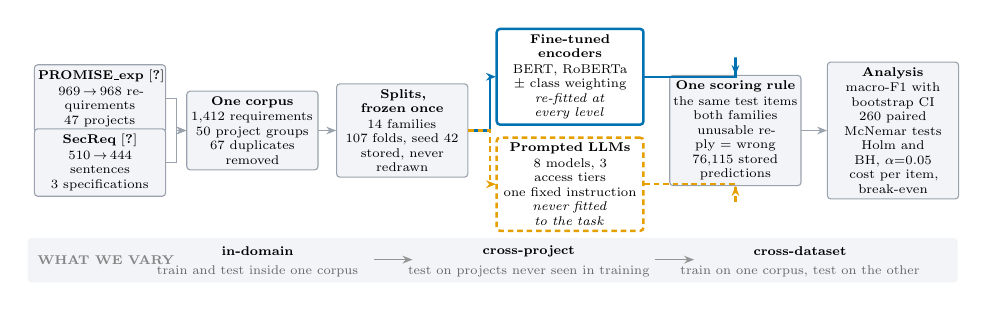
\begin{tikzpicture}[scale=0.81, transform shape,scale=0.81, transform shape,
  font=\footnotesize,
  >={Stealth[length=3.6pt,width=2.8pt]},
  bx/.style   ={draw=rule, line width=0.4pt, rounded corners=1.2pt, fill=white,
                align=center, text width=24mm, inner xsep=2pt, inner ysep=3pt,
                font=\scriptsize},
  src/.style  ={bx, fill=panel},
  enc/.style  ={bx, draw=encblue, line width=0.9pt, text width=27mm},
  llm/.style  ={bx, draw=llmgold, line width=0.9pt, dashed,
                dash pattern=on 2pt off 1.4pt, text width=27mm},
  ed/.style   ={->, draw=rule, line width=0.5pt},
  encd/.style ={->, draw=encblue, line width=0.9pt},
  llmd/.style ={->, draw=llmgold, line width=0.9pt, dashed,
                dash pattern=on 2pt off 1.4pt},
  tag/.style  ={font=\scriptsize, text=black!60, inner sep=1.2pt},
]
\def\cA{0}\def\cB{2.95}\def\cC{5.85}\def\cD{9.10}\def\cE{12.30}\def\cF{15.35}

%% --- the data path -------------------------------------------------------
\node[src] (s1)  at (\cA, 0.62) {\textbf{\pex{}}~\cite{lima2019}\\[0.5pt]
                                 969\,$\to$\,968 requirements\\47 projects};
\node[src] (s2)  at (\cA,-0.62) {\textbf{SecReq}~\cite{knauss2011}\\[0.5pt]
                                 510\,$\to$\,444 sentences\\3 specifications};
\node[src] (uni) at (\cB, 0)    {\textbf{One corpus}\\[0.5pt]1{,}412 requirements\\
                                 50 project groups\\67 duplicates removed};
\node[src] (spl) at (\cC, 0)    {\textbf{Splits, frozen once}\\[0.5pt]14 families\\
                                 107 folds, seed 42\\stored, never redrawn};

\draw[ed] (s1.east) -- ++(0.20,0) |- (uni.west);
\draw[ed] (s2.east) -- ++(0.20,0) |- (uni.west);
\draw[ed] (uni.east) -- (spl.west);

%% --- the two model families ----------------------------------------------
\node[enc] (fam1) at (\cD, 1.04) {\textbf{Fine-tuned encoders}\\[0.5pt]
                                  BERT, RoBERTa\\$\pm$ class weighting\\
                                  \emph{re-fitted at every level}};
\node[llm] (fam2) at (\cD,-1.04) {\textbf{Prompted LLMs}\\[0.5pt]
                                  8 models, 3 access tiers\\one fixed instruction\\
                                  \emph{never fitted to the task}};

\draw[encd] (spl.east) -- ++(0.42,0) |- (fam1.west);
\draw[llmd] (spl.east) -- ++(0.42,0) |- (fam2.west);

%% --- the shared scoring path ---------------------------------------------
\node[src] (sco) at (\cE, 0) {\textbf{One scoring rule}\\[0.5pt]the same test items\\
                              both families\\unusable reply $=$ wrong\\
                              76{,}115 stored predictions};
\node[src] (ana) at (\cF, 0) {\textbf{Analysis}\\[0.5pt]\Fm{} with bootstrap CI\\
                              260 paired McNemar tests\\Holm and BH, $\alpha{=}0.05$\\
                              cost per item, break-even};

\draw[encd] (fam1.east) -| ($(sco.north)+(0,0.34)$) -- (sco.north);
\draw[llmd] (fam2.east) -| ($(sco.south)-(0,0.34)$) -- (sco.south);
\draw[ed]   (sco.east) -- (ana.west);

%% --- the one thing we vary -----------------------------------------------
\begin{scope}[shift={(0,-2.52)}]
  \fill[panel, rounded corners=1.2pt] (-1.40,-0.42) rectangle (16.60,0.44);
  \node[font=\scriptsize\bfseries, text=black!48, anchor=west, align=left]
       at (-1.33,0.01) {WHAT WE VARY};
  \foreach \x/\name/\desc in {%
      3.05/{in-domain}/{train and test inside one corpus},
      8.30/{cross-project}/{test on projects never seen in training},
      13.55/{cross-dataset}/{train on one corpus, test on the other}}{%
      \node[font=\scriptsize, inner sep=0.8pt] at (\x,0.18) {\textbf{\name}};
      \node[tag] at (\x,-0.20) {\desc};}
  \draw[->, draw=black!42, line width=0.55pt] (5.30,0.02) -- (6.05,0.02);
  \draw[->, draw=black!42, line width=0.55pt] (10.75,0.02) -- (11.50,0.02);
\end{scope}
\end{tikzpicture}
\caption{How the experiment is put together. One data path on the left feeds two
families of model that differ in a single respect: whether they may learn from
labelled training data. The encoders (solid, upper) read the training folds and
are re-fitted at each level of the band beneath, so their scores move; the
prompted models (dashed, lower) read only the test items, so their scores cannot
move with the level, which makes them a fixed reference. Both families answer the
\emph{same} items --- which is what makes every encoder--LLM comparison a paired
one --- and both are marked by the same rule. The band is the only thing we
deliberately vary.}
\label{fig:arch}
\end{figure*}


\subsection{Data preparation}
\label{sec:data}
\pex{}~\cite{lima2019}, an expanded release of the PROMISE NFR collection,
contributes \nNpromise{} requirements from \nNpromiseProj{} projects, each
labelled FR or NFR and, when NFR, with one of eleven quality sub-types.
SecReq~\cite{knauss2011} contributes \nNsecreq{} sentences from \nNsecreqProj{}
industrial security specifications, each labelled security-relevant or not.

Preparation happens once, in the first stage. Texts are normalised and the label
strings mapped onto one controlled vocabulary, so both corpora express the
security concept in the same words. Exact duplicates are removed --- \nNdup{}
rows, all within a corpus rather than across the two --- taking the raw
\nNpromiseRaw{} and \nNsecreqRaw{} rows down to \nNtotal{} requirements in
\nNgroups{} project groups. The \nNsplitfam{} split families, \nNfolds{} folds in
all, are generated once with seed 42 and stored, keyed to identifiers pinned to
the SHA-256 hash of each source file; grouped-fold membership is library-version
dependent, so later stages read that file and never regenerate it.

Two properties of the prepared data matter throughout. The first is a difference
in class balance: security requirements are \nPrevPromise\% of \pex{} but
\nPrevSecreq\% of SecReq, a threefold difference in prevalence for a concept both
corpora annotate independently, and the cross-dataset regime is built on exactly
that contrast. The second is that the security label reaches the two corpora by
different routes. In \pex{} it comes from the security sub-class of the NFR
taxonomy, so every \pex{} item labelled security is also NFR and none of the
\nNfrPromise{} FRs is; in SecReq it applies to any security-relevant sentence,
and there is no FR/NFR annotation at all. The cross-dataset regime therefore
carries a shift in definition alongside the shift in distribution
(Section~\ref{sec:threats}). Because security is the only task both corpora
annotate, it is also the only task on which a cross-dataset comparison can be
posed at all.

\subsection{Tasks, label sets, and why they are not staged}
Binary FR/NFR uses the native \pex{} labels over all \nNpromise{} \pex{} items.
Binary security is native in SecReq and derived in \pex{}, which gives the same
task on two independently produced corpora. NFR sub-type classification uses the
eleven-class taxonomy of Cleland-Huang et al.~\cite{clelandhuang2007}, whose
categories align with the ISO/IEC 25010 quality characteristics~\cite{iso25010}.

The three tasks are evaluated independently, and the pipeline is not staged. The
security classifier is never shown the output of the FR/NFR classifier; every
item is presented to it directly, including the \nNfrPromise{} \pex{} items
labelled FR. We say this explicitly because the \pex{} annotation is
hierarchical, security being a sub-class of NFR, so it would be natural to assume
the pipeline is too. It is not, and deliberately so: a staged design would make
the security score depend on the errors of the FR/NFR classifier, and it would
have no counterpart in SecReq, where no FR/NFR labels exist.

Several sub-type classes have single-digit support, so that task is evaluated at
three granularities: eleven classes (\nNsubtypeall{} items), the six most
frequent (\nNsubtypesix) and the four most frequent (\nNsubtypefour). For an
encoder the label set fixes the size of the classification head, so the model is
re-trained for each granularity. A prompted model has no head to resize and no
training at all, so it is fair to ask what top-4 and top-6 can mean for it. They
change three things: the candidate labels are listed inside the prompt, so at
top-4 the model is offered four and at all-11 eleven; the evaluation frame
changes, since an item enters the top-4 frame only if its true label is one of
those four; and \Fm{} is computed over the full declared label set, so a model is
penalised for every declared class it never predicts. Granularity is a property
of the question and of the scoring, not of the model weights, which is why it is
measurable for both families.

\subsection{The three evaluation regimes}
\label{sec:regimes}
The \nNsplitfam{} frozen split families implement three levels of increasing
distribution shift, and this is the study's independent variable.
\emph{In-domain} is stratified 5-fold cross-validation within one corpus, the
setting essentially all prior work reports; it asks how well the model does on
more of the same data. \emph{Cross-project} uses grouped folds that hold out
entire project groups, plus a leave-one-project-out variant over the
\nNpromiseProj{} \pex{} projects; it asks how well the model does on a new
project inside a familiar corpus. \emph{Cross-dataset} fits on the security task
of one corpus and tests on the other, in both directions, with an identical label
set but a different annotation provenance; it asks the question a practitioner
actually faces, which is how well the model does on requirements written and
labelled by someone else.

The asymmetry between the families is the analytical lever. The encoders are
re-fitted at every regime on that regime's training folds, so their scores move;
the prompted models have no training distribution to shift, so their scores
cannot move with the regime, which is why a single value is written across the
regime columns of Table~\ref{tab:main} for each of them. That fixed reference is
what lets the encoders' loss be attributed to the shift rather than to the
difficulty of the items. Every requirement is a test item exactly once within
each encoder family; the prompted models answer stratified samples of the same
items (300 per binary cell, 200 per sub-type cell, in proportion to the class
prior with a floor of ten per class), and the six local models additionally
answer the full frames.

\subsection{The two model families, and why they are compared}
\label{sec:families}
Table~\ref{tab:configs} lists the twelve configurations, and the architectural
difference between them is not incidental to the question. A fine-tuned encoder
is a bidirectional, encoder-only transformer, pre-trained with masked language
modelling and then adapted by supervised training of a classification head over
the pooled sentence representation, so both its decision boundary and its class
prior are learned from the labelled training folds. A prompted LLM is a
decoder-only autoregressive model never adapted to the task: it receives the
label vocabulary as text, answers in generated tokens, and its implicit class
prior comes from pre-training and from the instruction rather than from any
corpus of requirements. That contrast is what makes the comparison informative,
because the two families should react differently to a shift in distribution
precisely by acquiring their prior in different places, and
Section~\ref{sec:mechanism} shows that they do. Prior work has argued that
architecture affects results on this task~\cite{vasudevan2026}, so we treat it as
a declared property and report every result per configuration.

We fine-tune \texttt{bert-\allowbreak base-\allowbreak uncased}~\cite{devlin2019} and
\texttt{roberta-\allowbreak base}~\cite{liu2019} with a classification head (AdamW, lr
$2\times10^{-5}$, batch 16, max length 128; 3 epochs on the binary tasks, 10 on
the sub-types), each with inverse-frequency class weighting, plus an unweighted
control on the security task. The local tier runs six instruction-tuned models of
2.6--8.0\,B parameters on a single free-tier NVIDIA T4 under 4-bit NF4
quantisation~\cite{dettmers2023}; the hosted and commercial tiers reach
Llama-3.3-70B and Gemini 3.1 Flash-Lite through free API tiers. A ninth prompted
model failed the gate of Section~\ref{sec:scoring} and enters no table.

\begin{table}[t]
\caption{The twelve model configurations. ``B'' is the published parameter count
of the exact checkpoint, in billions; Gemini's is undisclosed and is recorded as
unknown rather than estimated.}
\label{tab:configs}
\centering
\scriptsize
\setlength{\tabcolsep}{4pt}
\renewcommand{\arraystretch}{1.02}
\begin{tabular}{@{}llcl@{}}
\toprule
\textbf{Configuration} & \textbf{Checkpoint / endpoint} & \textbf{B} & \textbf{Access} \\
\midrule
BERT (w / u)        & \texttt{bert-base-uncased}     & 0.11 & fine-tuned \\
RoBERTa (w / u)     & \texttt{roberta-base}          & 0.13 & fine-tuned \\
\addlinespace[1.5pt]
Gemma-2-2B          & \texttt{gemma-2-2b-it}         & 2.61 & local, 4-bit \\
SmolLM3-3B          & \texttt{SmolLM3-3B}            & 3.08 & local, 4-bit \\
Qwen2.5-3B          & \texttt{Qwen2.5-3B-Instruct}   & 3.09 & local, 4-bit \\
Phi-4-mini          & \texttt{Phi-4-mini-instruct}   & 3.84 & local, 4-bit \\
Qwen2.5-7B          & \texttt{Qwen2.5-7B-Instruct}   & 7.62 & local, 4-bit \\
Llama-3.1-8B        & \texttt{Llama-3.1-8B-Instruct} & 8.03 & local, 4-bit \\
\addlinespace[1.5pt]
Llama-3.3-70B       & \texttt{llama-3.3-70b-versatile} & 70.6 & hosted \\
Gemini 3.1 F-Lite   & \texttt{gemini-3.1-flash-lite} & n/a  & commercial \\
\bottomrule
\end{tabular}
\end{table}

\subsection{The prompt, and why it is fixed}
\label{sec:prompt}
Each prompted model answers a fixed instruction that names the task, lists the
label vocabulary and requires exactly one word in reply, sent as a single user
message. Decoding is greedy, temperature 0 with at most twelve new tokens, so the
only stochastic element left is which items are sampled. The base FR/NFR
instruction is reproduced below; the sub-type tasks use the same template with
the permitted labels listed in place of ``FR''/``NFR'', which is how the top-4,
top-6 and all-11 variants differ for a prompted model.

{\scriptsize\ttfamily\raggedright
\vspace{2pt}\noindent\hrulefill\\[1.5pt]
You are classifying a software requirement.\\
Decide whether it is a FUNCTIONAL requirement (FR) --\\
something the system must DO -- or a NON-FUNCTIONAL\\
requirement (NFR), a quality, constraint or property\\
such as performance, security or usability.\\
Answer with exactly one word: "FR" or "NFR".\\[1.5pt]
$\langle$few-shot only: k exemplars here$\rangle$\\[1.5pt]
Requirement: """the requirement under test"""\\
Answer:\\[1.5pt]
\noindent\hrulefill\vspace{2pt}}

Fixing the instruction needs justifying, because a different wording could give a
different result and a better one almost certainly exists. The template follows
the zero-shot format used by the studies we compare
against~\cite{binkhonain2025,alhoshan2025,tang2025}: a task statement, a list of
permitted labels, and an instruction to answer with the label alone. We did not
tune it against the test items. The design requires a \emph{fixed} instruction so
that the only quantity varying across the three regimes is the distribution
shift; re-optimising the wording per regime would make any difference between
regimes unattributable to the shift, which is the one thing this study sets out
to measure. The prompt is a control, not a recommendation.

What a better wording would be worth is measured rather than assumed. A sub-study
re-runs two models over three phrasings of the same question (base, terse and
verbose) with the answer contract held identical, over \nNpsCells{} paired cells.
An oracle picking the best wording per cell would gain a median of \nOracleMed{}
\Fm{} and at most \nOracleMax{} --- far less than the differences our conclusions
rest on, and picking it would require labelled data from the target corpus, the
very resource prompting is meant to do without. A second sub-study is a few-shot
ladder ($k \in \{2,4,8\}$ on the binary tasks, $k \in \{1,2\}$ per class on the
sub-types) with class-balanced exemplars carved out before the evaluation frames
are formed, so an exemplar is never also a test item.

\subsection{Scoring, and how to read the numbers}
\label{sec:scoring}
Replies are parsed by a strict, word-boundary-aware rule: a leading label wins;
otherwise exactly one label named anywhere in the reply wins; a reply naming both
labels or neither is unusable and is scored as wrong. This is harsher than the
lenient protocols common in prior work, and it matches deployment, where an
unusable answer is not a free pass. The rule runs at generation time and again in
an idempotent repair pass over the archived outputs, so stored and scored
predictions cannot drift apart. Encoder rows are argmax predictions and are
exempt from the parse-rate gate.

Four kinds of quantity appear in this paper. They are easy to confuse, so we say
what each one is and name it explicitly at every use.

\begin{itemize}\itemsep0.5pt \parskip0pt \topsep2pt
\item \textbf{\Fm{}}: the unweighted mean of the per-class F1 scores over the
      full declared label set, on a 0--1 scale. It is primary because it does not
      let a model score well by ignoring a rare class; the majority-class
      baseline in the last row of Table~\ref{tab:main} gives it a floor.
\item \textbf{Relative loss} ($\Delta\%$): the share of a configuration's
      \emph{own} in-domain \Fm{} that it loses in a shifted regime, on the same
      items. Only the encoders have it, because only they have a fit to lose.
\item \textbf{Predicted class share}: the fraction of test items a model assigns
      to a class. Not an accuracy --- it is what the model takes the class
      balance to be, read against the true prevalence in the same items.
\item \textbf{Test counts}: numbers of statistical comparisons, not of
      requirements. One unit is one exact McNemar test between one encoder and
      one prompted model in one cell.
\end{itemize}

Uncertainty uses a stratified bootstrap of 2,000 resamples within each true class
(seed 42). Encoder--LLM comparisons use the exact two-sided McNemar test on
paired disagreements~\cite{mcnemar1947}, and all \nNtests{} are corrected as one
family under Holm~\cite{holm1979} and Benjamini--Hochberg~\cite{bh1995} at
$\alpha = 0.05$, with verdicts keyed on the BH-adjusted $p$ (\nSigRaw{}
significant before correction, \nSigBH{} after BH, \nSigHolm{} after Holm). A
cell --- one model, task, dataset and regime --- is reported only if every class
has at least five test items, the cell holds at least 40 items, and the model
parsed at least half of its responses; \nNcellsdrop{} of \nNcells{} cells fail
that gate and are excluded rather than imputed. The store holds \nNpred{} rows.

\subsection{How cost is computed}
\label{sec:cost}
Every prediction row records token counts, wall-clock latency and, for the
encoders, training time, so cost is computed from recorded quantities rather than
estimated after the fact. The basis differs by tier, because the two kinds of
model are billed differently.

\emph{Models that run on our own hardware are priced on compute.} That covers the
encoders and all six local open-weight models: they are free to download and
carry no licence fee, so the only thing to charge for is the machine time they
occupy. We price it as an imputed rental of the benchmark GPU --- an AWS
g4dn.xlarge with one NVIDIA T4, at the published on-demand list rate for
us-east-1 of \$\nGpuOnDemand{} per hour, recorded in the manifest with the date
it was checked (\nGpuSource). That is a list price for hardware, not for the
model, and it assumes unbatched inference; the stored sensitivity table reports
the same costs at the spot rate (\$\nGpuSpot/h) and at batch sizes 8 and 32,
which cut the local figures by roughly an order of magnitude.

\emph{Models behind an API are priced on tokens}, at the provider's published
list rate per million input and output tokens: \$\nPriceGemIn/\$\nPriceGemOut{}
for Gemini 3.1 Flash-Lite and \$\nPriceLlaIn/\$\nPriceLlaOut{} for
Llama-3.3-70B, taken from the providers' public rate cards in August 2026 and
frozen into every prediction row at generation time, so a later price change
cannot alter a stored result. Both were in fact run on free tiers; the list rate
is what the same volume would have cost.

Neither basis is a fixed property of the technique, and cost should be expected
to move with model size and capability. Within the compute-priced tier it plainly
does: over the \nNlocalCfg{} locally executed configurations, cost per item rises
with parameter count (Spearman $\rho = \nRhoSize$). That is why
Section~\ref{sec:rqthree} states the comparison as a ratio between tiers rather
than an absolute price that would date. Encoder cost separates the one-off
training cost $C_0$ from the marginal per-item cost $c_\text{enc}$, giving a
break-even volume against any prompted alternative of marginal cost
$c_\text{alt}$:
\begin{equation}
N^{\star} = \frac{C_0}{c_\text{alt} - c_\text{enc}}
\label{eq:breakeven}
\end{equation}
Because free-tier latency is dominated by queueing on the provider's side,
wall-clock projections use the per-request median latency, not the mean.

%% ===========================================================================
\section{Results}
\label{sec:results}
%% ===========================================================================
Table~\ref{tab:main} is the paper's single results table: all twelve
configurations, the six task-by-corpus cells and every regime each supports, so
that encoders and prompted models are read off the same rows and columns. The
encoders have one score per regime because they are re-fitted at each; a prompted
model has one score per cell, written across the regime columns it spans, because
a model that consumes no training data cannot score differently when that data
changes.

\begin{table*}[t]
\caption{\Fm{} for all twelve configurations, across every task, corpus and
regime. ID = in-domain, XP = cross-project, XD = cross-dataset. Best per column
in bold; ``--'' marks a cell below the reportability gate of
Section~\ref{sec:scoring}, or a regime that does not apply. A prompted model's
score is written once across the regimes of its cell, because it consumes no
training data and the regime cannot move it. Encoder cells are cross-validated
over all items ($n = \nNcellItems{}$ by task group); prompted cells are
stratified samples of them ($n = \nNpromptMin$--$\nNpromptMax$).}
\label{tab:main}
\centering
\setlength{\tabcolsep}{3.0pt}
\renewcommand{\arraystretch}{1.05}
\begin{tabular}{@{}l*{14}{c}@{}}
\toprule
& \multicolumn{6}{c}{\textbf{Security}} & \multicolumn{2}{c}{\textbf{FR/NFR}} & \multicolumn{6}{c}{\textbf{NFR sub-types} (\pex{})} \\
\cmidrule(lr){2-7}\cmidrule(lr){8-9}\cmidrule(l){10-15}
& \multicolumn{3}{c}{\pex{}} & \multicolumn{3}{c}{SecReq} & \multicolumn{2}{c}{\pex{}} & \multicolumn{2}{c}{top-4} & \multicolumn{2}{c}{top-6} & \multicolumn{2}{c}{all-11} \\
\cmidrule(lr){2-4}\cmidrule(lr){5-7}\cmidrule(lr){8-9}\cmidrule(lr){10-11}\cmidrule(lr){12-13}\cmidrule(l){14-15}
\textbf{Configuration} & \ID & \XP & \XD & \ID & \XP & \XD & \ID & \XP & \ID & \XP & \ID & \XP & \ID & \XP \\
\midrule
BERT\textsubscript{w} & \textbf{0.923} & 0.865 & 0.528 & 0.836 & 0.588 & 0.690 & \textbf{0.908} & 0.843 & 0.878 & 0.800 & 0.827 & 0.735 & 0.657 & 0.579 \\
BERT\textsubscript{u} & 0.907 & -- & 0.534 & -- & -- & 0.702 & -- & -- & -- & -- & -- & -- & -- & -- \\
RoBERTa\textsubscript{w} & 0.902 & 0.876 & 0.698 & 0.824 & 0.668 & 0.696 & 0.896 & 0.853 & \textbf{0.936} & 0.835 & \textbf{0.837} & 0.753 & \textbf{0.724} & \textbf{0.688} \\
RoBERTa\textsubscript{u} & 0.903 & -- & 0.707 & -- & -- & 0.678 & -- & -- & -- & -- & -- & -- & -- & -- \\
\addlinespace[1.5pt]
Gemini 3.1 Flash-Lite & \multicolumn{3}{c}{0.829} & \multicolumn{3}{c}{0.713} & \multicolumn{2}{c}{0.867} & \multicolumn{2}{c}{0.922} & \multicolumn{2}{c}{--} & \multicolumn{2}{c}{--} \\
Llama-3.3-70B & \multicolumn{3}{c}{0.891} & \multicolumn{3}{c}{0.814} & \multicolumn{2}{c}{0.852} & \multicolumn{2}{c}{0.907} & \multicolumn{2}{c}{0.782} & \multicolumn{2}{c}{--} \\
\addlinespace[1.5pt]
Qwen2.5-7B & \multicolumn{3}{c}{0.884} & \multicolumn{3}{c}{\textbf{0.846}} & \multicolumn{2}{c}{0.656} & \multicolumn{2}{c}{0.876} & \multicolumn{2}{c}{0.824} & \multicolumn{2}{c}{0.576} \\
Llama-3.1-8B & \multicolumn{3}{c}{0.872} & \multicolumn{3}{c}{0.845} & \multicolumn{2}{c}{0.682} & \multicolumn{2}{c}{0.700} & \multicolumn{2}{c}{0.717} & \multicolumn{2}{c}{0.629} \\
Gemma-2-2B & \multicolumn{3}{c}{0.900} & \multicolumn{3}{c}{0.821} & \multicolumn{2}{c}{0.663} & \multicolumn{2}{c}{0.760} & \multicolumn{2}{c}{0.603} & \multicolumn{2}{c}{0.527} \\
Phi-4-mini & \multicolumn{3}{c}{0.798} & \multicolumn{3}{c}{0.635} & \multicolumn{2}{c}{0.727} & \multicolumn{2}{c}{0.727} & \multicolumn{2}{c}{0.712} & \multicolumn{2}{c}{0.599} \\
SmolLM3-3B & \multicolumn{3}{c}{0.841} & \multicolumn{3}{c}{0.717} & \multicolumn{2}{c}{0.562} & \multicolumn{2}{c}{0.763} & \multicolumn{2}{c}{0.693} & \multicolumn{2}{c}{0.482} \\
Qwen2.5-3B & \multicolumn{3}{c}{0.707} & \multicolumn{3}{c}{0.741} & \multicolumn{2}{c}{0.554} & \multicolumn{2}{c}{0.732} & \multicolumn{2}{c}{0.689} & \multicolumn{2}{c}{0.543} \\
\midrule
\textit{majority-class baseline} & \multicolumn{3}{c}{0.466} & \multicolumn{3}{c}{0.376} & \multicolumn{2}{c}{0.351} & \multicolumn{2}{c}{0.131} & \multicolumn{2}{c}{0.075} & \multicolumn{2}{c}{0.035} \\
\bottomrule
\end{tabular}

\end{table*}

\subsection{RQ1: within one corpus, supervision is still ahead}
Reading the ID columns of Table~\ref{tab:main}, the fine-tuned encoders hold the
best score in five of the six cells: class-weighted BERT on FR/NFR and on \pex{}
security, class-weighted RoBERTa on all three sub-type granularities. The
exception is SecReq security, where 4-bit Qwen2.5-7B posts the better point
estimate (\nSecreqBestLLM{} against \nSecreqBestEnc), a lead that does not reach
significance (exact McNemar $p = \nSecreqP$; BH-adjusted \nSecreqPBH).

Three observations qualify that ranking. Scale does not order the results: the
2.6\,B Gemma-2-2B scores \nGemmaSec{} on \pex{} security against \nLlamaSec{} for
the hosted 70\,B model. The encoder advantage widens as the label set grows, from
\nLeadFour{} \Fm{} on top-4 to \nLeadAll{} on all-11 over the best prompted
model, as expected if supervision mainly buys the long tail of rare classes. And
because cell sizes differ, the top-4 ranking was recomputed on the
\nNcommonFour{} items every model answered; the best encoder still leads there by
\nLeadFourCommon{} \Fm{}, so the ordering is not an artefact of coverage. Over
the \nNtestID{} in-domain comparisons the encoders win \nWinID{} and lose none,
the remaining \nTieID{} being inconclusive (Fig.~\ref{fig:inv}(b)).

\subsection{RQ2: the ranking reverses under distribution shift}
\label{sec:rqtwo}

\begin{figure}[t]
\centering
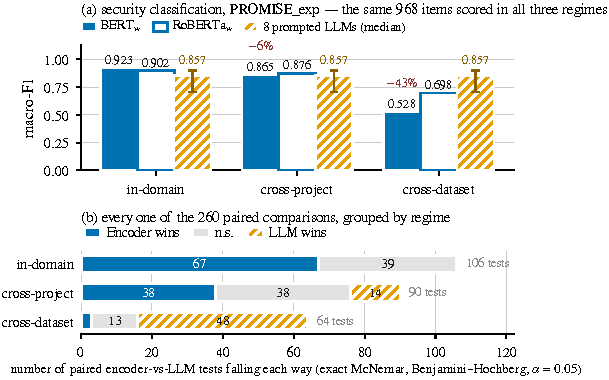
\includegraphics[width=\columnwidth]{figures/fig_inversion.pdf}
\caption{(a) Security classification on \pex{}. All bars are scored on the same
\nNpromise{} items at every level; the encoders are re-fitted at each level,
while the third bar (median of the eight prompted models, whisker = their full
range) is flat because those models are never fitted. The red annotation is a
\emph{relative loss of \Fm{}} --- BERT's cross-dataset score is \nDropXDmax\%
below its own in-domain score --- not a share of items. (b) The \nNtests{} paired
comparisons, grouped by the regime the encoder was evaluated under. One unit on
the axis is one McNemar test, not one requirement.}
\label{fig:inv}
\end{figure}

\emph{Cross-project transfer is survivable.} Holding out unseen projects costs
the encoders \nDropXPpromMin--\nDropXPpromMax\% of their in-domain \Fm{} on
\pex{}, and at most \nDropXPmax\% anywhere in this regime (BERT on SecReq, whose
three project groups make a held-out group a third of the corpus). They stay
ahead or tied in \nAheadXP{} of the \nNtestXP{} paired tests: the degradation
NoRBERT anticipated~\cite{hey2020norbert}, real but moderate.

\emph{Cross-dataset transfer reverses the ranking.} The class-weighted BERT that
scores \nXDrefF{} on \pex{} security falls to \nXDtransF{} on the same items once
its training corpus is swapped for SecReq. That is \nDropXDmax\% of its in-domain
\Fm{}, the largest relative loss in the study; it belongs to the cross-dataset
regime and should not be read against the cross-project figures above, whose
largest value is \nDropXPmax\%. RoBERTa is more robust ($-\nDropXDRw\%$), the
unweighted controls behave like their weighted counterparts ($-\nDropXDBu\%$ and
$-\nDropXDRu\%$), and the reverse direction is milder still ($-\nDropXDrevMin\%$
to $-\nDropXDrevMax\%$). The prompted models, having nothing to re-fit, move only
with the difficulty of the corpus. Over the \nNtestXD{} cross-dataset comparisons
they win \nLossXD{} and the encoders \nWinXD{}: the in-domain tally of
\nWinID--\nTieID--\nLossID{} becomes \nWinXD--\nTieXD--\nLossXD{}, on the same
twelve models and the same scorer.

\emph{Corpus-level averages hide per-project failure.} On the
leave-one-project-out variant of FR/NFR, over the \nNppProj{} projects with
comparable coverage, every configuration scores 0.000 on at least one project and
1.000 on another. Only the middle separates them: the encoders' median
per-project accuracy is \nPpEncMed{} against \nPpLocMedMin--\nPpLocMedMax{} for
the small open models.

\subsection{The cause is a mis-set class balance, in both families}
\label{sec:mechanism}

\begin{figure}[t]
\centering
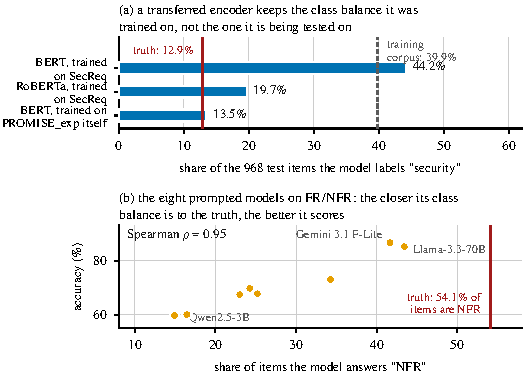
\includegraphics[width=\columnwidth]{figures/fig_prior.pdf}
\caption{One failure mode reached by two routes. (a) The share of the
\nNpromise{} \pex{} test items each encoder labels \emph{security} --- a share of
items, not a score. Red line: the true share in those items. Grey line: the share
in SecReq, the corpus the transferred models were trained on. (b) The eight
prompted models on FR/NFR; the horizontal axis is again a share of items and each
point is one model.}
\label{fig:prior}
\end{figure}

A drop in score does not by itself say why a model failed, and the two candidate
explanations imply different remedies. If the transferred encoder fails because
the new corpus uses unfamiliar vocabulary, the fix is more or broader training
text; if it fails because it has the wrong idea of how common the class is, the
fix is a prior correction, which needs no labels from the target corpus at all.
The per-class evidence separates the two (Fig.~\ref{fig:prior}).

After transfer from SecReq, BERT labels \nShareBertXD\% of the \pex{} items
\emph{security}, against a true prevalence of \nPrevPromise\% in those items and
\nPrevSecreq\% in the corpus it was trained on. That \nShareBertXD\% is a
predicted class share, not a loss of score; its closeness to the \nDropXDmax\%
quoted above is a coincidence of arithmetic, and the two must not be read
together. The consequence is visible per class: precision on the security class
falls from \nPrecID{} to \nPrecXD{} while recall falls far less, from \nRecID{}
to \nRecXD{}. The model still finds the security requirements; what it cannot do
is stop finding them, which is the signature of a shifted prior rather than a
failure to read the text. The picture is not uniform --- RoBERTa carries less of
its source prior across (\nShareRobXD\% against \nPrevPromise\% true) and loses
correspondingly less --- but the dominant term in the largest observed collapse
is a prior the model brought with it, which is an encouraging diagnosis: prior
shift is correctable without labels from the target
corpus~\cite{saerens2002}.

Turning the same instrument on the prompted models finds the same defect arriving
by a different route. On FR/NFR the true NFR share is \nShareNFR\%, and every
prompted model predicts NFR less often, from \nLLMnfrMin\% (\nLLMnfrMinModel) to
\nLLMnfrMax\% (Llama-3.3-70B). Their accuracies rank almost exactly with that
miscalibration (Spearman $\rho = \nRhoPrior$, Fig.~\ref{fig:prior}(b)), so the
weak FR/NFR scores of the small open models reflect a systematic bias towards
answering FR, not an inability to read the requirement.

The wording of the question moves that balance directly, which makes the link
causal rather than merely correlational. Across the \nNpsCells{} paired cells of
the phrasing sub-study the median spread between the three wordings is
\nSpreadMed{} \Fm{}, but the largest is \nSpreadMax{}, for Gemma-2-2B on SecReq
security: the terse variant is the only one phrased as a leading yes/no question,
and under it Gemma-2-2B answers \emph{security} for \nTerseShare\% of SecReq
items against a true rate of \nTerseTrue\%. This is not a formatting artefact,
since the parser accepted \nPsParse\% of the sub-study's \nNpsRows{} responses.
Prompt sensitivity is itself well documented~\cite{zhao2021}; what is new is that
it lands on the same failure mode as the encoders' transfer loss. Few-shot
exemplars help only where they carry information about the class balance: over
the \nNfsTests{} paired comparisons the median gain is \nFsMed{} \Fm{}, negative
on the binary tasks (mean \nFsBinMean{}) and positive on the sub-types (mean
\nFsSubMean{}), the over-prompting effect Tang et al.\ report~\cite{tang2025}.
This is one defect with two sources: the task needs a class prior that cannot be
read off the requirement text, and each family takes one from somewhere it should
not.

\subsection{RQ3: the accuracy--cost trade-off}
\label{sec:rqthree}

\begin{figure}[t]
\centering
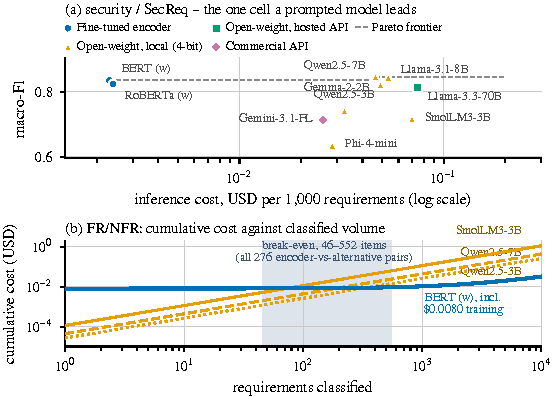
\includegraphics[width=\columnwidth]{figures/fig_cost.pdf}
\caption{(a) Price of 1,000 classifications, on the basis of
Section~\ref{sec:cost}: compute time for anything run on our own GPU, published
token rates for the two API models. (b) Total cost against volume for one
encoder--LLM pair. The encoder starts above zero because it must be trained once;
the prompted model starts at zero and rises faster. The crossing point is
$N^{\star}$ from~(\ref{eq:breakeven}).}
\label{fig:cost}
\end{figure}

Encoder inference costs \$\nCostEnc{} per 1,000 classifications on the imputed T4
rental of Section~\ref{sec:cost}. The prompted configurations range from
\$\nCostLLMmin{} to \$\nCostLLMmax{} per 1,000 on the same basis, taking each
model's median across its cells: \nRatioMin{} to \nRatioMax{} times the encoder,
about \nRatioMed{} times at the medians (Fig.~\ref{fig:cost}(a)). One-off
fine-tuning is small, a median of \$\nTrainMed{} per deployable model
(\nTrainSec{} GPU-seconds over all folds of a family), so the break-even
of~(\ref{eq:breakeven}) arrives quickly: over all \nNBE{} encoder--LLM pairings
$N^{\star}$ lies between \nBEmin{} and \nBEmax{} items, median \nBEmed{}. In
concrete terms, classifying 10,000 requirements costs \$\nTenkEnc{} with a
fine-tuned encoder, \$\nTenkGem{} with the commercial API and \$\nTenkLla{} with
the hosted 70\,B model. The Pareto frontier holds \nNPareto{} cells,
\nNParetoEnc{} of them encoders; the one prompted frontier point is 4-bit
\nParetoLLM{} on SecReq security, which buys \nParetoGain{} \Fm{} for roughly
\nParetoRatio$\times$ the cost per item.

Two qualifications keep these figures in proportion: they are ratios measured on
one machine at one date, and the model prices computation only, so the annotation
an encoder needs is excluded, which favours the encoder. Latency behaves
differently --- \nLatEnc\,s median per request for the encoders, \nLatHost\,s
for the hosted 70\,B model, \nLatLocMin--\nLatLocMax\,s for the local open
models and \nLatCom\,s for the commercial API.

%% ===========================================================================
\section{Discussion}
%% ===========================================================================
\subsection{Generalisability}
The most consequential result is not that one family is better than the other,
but that the answer to ``which is better?'' changes between two protocols the
literature treats as interchangeable, on the same corpora, items and scorer. A
benchmark reporting only in-distribution numbers is not a weaker version of one
that reports transfer; on this evidence it can report the opposite ordering. Two
things follow: the regime belongs in the claim, next to the metric; and
``generalisation'' should mean held-out projects or an independently annotated
corpus, not transfer across tasks within one dataset~\cite{binkhonain2025}. The limits of our own claim are equally explicit:
we observe the reversal on one corpus pair, one task and one language, so the
study shows that it is possible and large when it happens, not that it occurs at
any particular rate. The mechanism we identify is what would make it recur, and
it is checkable on any new pair without re-running our models --- compare the
share of items a model assigns to the rare class against the prevalence of that
class in the target data, and if the two disagree badly the score will follow.

\subsection{Consistency and reliability}
Accuracy averaged over a corpus is not the only property a practitioner needs,
and two kinds of instability appear here, one per family. The encoders are stable
given a fixed training distribution and unstable when it moves: their scores
change little across folds inside a corpus, but they lose up to \nDropXDmax\% of
their in-domain \Fm{} when the training corpus is replaced. That failure is at
least predictable before deployment, from the class balance of the corpus they
were fitted on relative to the target. The prompted models are stable across
regimes by construction but unstable with respect to the question: re-wording the
same instruction, with the answer contract held fixed, moved \Fm{} by up to
\nSpreadMax{} in one cell. Pinning the prompt gives repeatable answers, but the
level at which they repeat was set by a wording choice no in-distribution study
would surface. Both families also show wide per-project variance.

\subsection{The accuracy--cost trade-off in practice}
For a team with a few hundred labelled requirements from the domain it will
actually operate in, and any non-trivial volume of work, a fine-tuned encoder of
about 110\,M parameters is both the more accurate and much the cheaper option.
Entering an unlabelled or shifting domain changes the answer: a mid-size
quantised open model gives up some in-domain accuracy, degrades far more
gracefully, and runs on one consumer-class GPU without an API contract. What the
results argue against is the implicit default of much recent work: fine-tuning on
one corpus and assuming the result transfers.

\subsection{Contamination and availability}
Both corpora are old, small and public, so prompted in-domain scores may be
inflated by pre-training contamination~\cite{sainz2023}. That bias would
overstate the prompted models in-domain, which is where we report the encoders
winning, so the in-domain advantage is conservative; and it cannot produce the
cross-dataset reversal, because it would help them equally in both regimes. The
pipeline, the splits, the prediction store and the scripts that regenerate every
table and figure will be released, and scoring is a pure function of the stored
outputs, so every number reproduces without re-running a model.

%% ===========================================================================
\section{Threats to Validity}
\label{sec:threats}
%% ===========================================================================
\emph{Internal.} The commercial tier ran at about \nNGemini{} items per cell,
where \nTieGemini{} of its \nNtestGemini{} paired comparisons are inconclusive,
so ``never significantly beaten'' partly reflects limited statistical power.
Free-tier quotas caused missing-not-at-random dropout on some hosted
configurations; the gate excludes the affected cells rather than imputing them.
Local models ran 4-bit quantised, and each configuration used a single seed.

\emph{Construct.} GPU costs are imputed from a published rental rate rather than
billed, and token prices are 2026 list rates, so the ratios are more durable than
the absolute values. $N^{\star}$ is a cost crossover computed regardless of the
accuracy gap, and strict scoring counts format non-compliance as error, which
matches deployment but differs from some prior protocols.

\emph{External.} Both corpora are small, dated and public, and their security
label sets differ (Section~\ref{sec:data}), so the cross-dataset regime carries
definitional as well as distributional shift, on one corpus pair. Results cover
English requirements and one NFR taxonomy.

%% ===========================================================================
\section{Conclusion}
%% ===========================================================================
We compared four fine-tuned encoder configurations against eight prompted LLMs on
three requirements-classification tasks, holding the items, the label sets and
the scoring rule fixed and varying only the distance between the data a model was
fitted on and the data it was scored on. Within a corpus the encoders are ahead
and are never significantly beaten; across an independently annotated corpus the
ordering reverses, while the encoders remain an order of magnitude cheaper per
item and repay their training after a few hundred classifications. The cause is
the same in both families: a class prior acquired from somewhere other than the
corpus being classified. An in-distribution score is therefore not a partial
answer to the question of which approach to adopt --- it can be the wrong one.

Two extensions follow from the design. Parameter-efficient fine-tuning of the
LLMs, with LoRA adapters over the same 4-bit checkpoints~\cite{dettmers2023},
would let a prompted model be re-fitted at each regime exactly as the encoders
are, separating whether prompted models transfer better because they are
decoder-only or simply because they were never fitted to a source corpus;
Section~\ref{sec:mechanism} predicts the latter. A third independently annotated
corpus such as PURE~\cite{ferrari2017} would turn one cross-dataset contrast into
several and let the prevalence gap be varied rather than merely observed, so that
prior adjustment~\cite{saerens2002} could be evaluated as a remedy rather than
left, as here, as a diagnosis.

\balance
%% ===========================================================================
\begin{thebibliography}{99}
\setlength{\itemsep}{0pt plus 0.3pt}
\bibitem{clelandhuang2007} J. Cleland-Huang et al., ``Automated classification of
non-functional requirements,'' \emph{Requirements Eng.}, vol.~12, no.~2,
pp.~103--120, 2007.
\bibitem{iso29148} ``ISO/IEC/IEEE International Standard --- Systems and
software engineering --- Life cycle processes --- Requirements engineering,''
in \emph{ISO/IEC/IEEE 29148:2018(E)}, pp.~1--104, 30 Nov. 2018,
doi: 10.1109/IEEESTD.2018.8559686.
\bibitem{kurtanovic2017} Z. Kurtanovi\'c and W. Maalej, ``Automatically
classifying functional and non-functional requirements using supervised machine
learning,'' in \emph{Proc. IEEE RE}, 2017, pp.~490--495.
\bibitem{hey2020norbert} T. Hey et al., ``NoRBERT: Transfer learning for
requirements classification,'' in \emph{Proc. IEEE RE}, 2020, pp.~169--179.
\bibitem{alhoshan2023} W. Alhoshan, A. Ferrari, and L. Zhao, ``Zero-shot
learning for requirements classification: An exploratory study,''
\emph{Inf. Softw. Technol.}, vol.~159, art.~107202, 2023.
\bibitem{elhajjami2024} A. El-Hajjami, N. Fafin, and C. Salinesi, ``Which AI
technique is better to classify requirements? An experiment with SVM, LSTM, and
ChatGPT,'' arXiv:2311.11547, 2024.
\bibitem{kaur2024} K. Kaur and P. Kaur, ``The application of AI techniques in
requirements classification: A systematic mapping,'' \emph{Artif. Intell.
Rev.}, vol.~57, art.~57, 2024, doi: 10.1007/s10462-023-10667-1.
\bibitem{peer2024} J. Peer, Y. Mordecai, and Y. Reich, ``NLP4ReF: Requirements
classification and forecasting --- From model-based design to large language
models,'' in \emph{Proc. IEEE Aerospace Conf.}, 2024, pp.~1--16.
\bibitem{binkhonain2025} M. Binkhonain and R. Alfayaz, ``Are prompts all you
need? Evaluating prompt-based large language models for software requirements
classification,'' \emph{Requirements Eng.}, 2025.
\bibitem{alhoshan2025} W. Alhoshan, A. Ferrari, and L. Zhao, ``How effective
are generative large language models in performing requirements
classification?'' arXiv:2504.16768, 2025.
\bibitem{tang2025} Y. Tang et al., ``The few-shot dilemma: Over-prompting large
language models,'' arXiv:2509.13196, 2025.
\bibitem{chaudhary2025} M. Chaudhary, C. Jain, and P. R. Anish, ``Exploring
zero-shot app review classification with ChatGPT: Challenges and potential,''
arXiv:2505.04759, 2025.
\bibitem{vasudevan2026} P. Vasudevan et al., ``Requirements classification using
fine-tuned transformer models: A comparative study of BERT, RoBERTa, and
GPT-4o,'' in \emph{Proc. ACM Southeast Conf. (ACMSE)}, 2026, pp.~199--204.
\bibitem{levy2026} O. Levy et al., ``AI-assisted requirements engineering: An
empirical evaluation relative to expert judgment,'' arXiv:2604.15222, 2026.
\bibitem{knauss2011} E. Knauss et al., ``Supporting requirements engineers in
recognising security issues,'' in \emph{Proc. REFSQ}, 2011, pp.~4--18.
\bibitem{lima2019} M. Lima et al., ``Software engineering repositories: Expanding
the PROMISE database,'' in \emph{Proc. SBES}, 2019, pp.~427--436.
\bibitem{ferrari2017} A. Ferrari, G. O. Spagnolo, and S. Gnesi, ``PURE: A dataset
of public requirements documents,'' in \emph{Proc. IEEE RE}, 2017,
pp.~502--505.
\bibitem{devlin2019} J. Devlin et al., ``BERT: Pre-training of deep bidirectional
transformers for language understanding,'' in \emph{Proc. NAACL-HLT}, 2019,
pp.~4171--4186.
\bibitem{liu2019} Y. Liu et al., ``RoBERTa: A robustly optimized BERT
pretraining approach,'' arXiv:1907.11692, 2019.
\bibitem{dettmers2023} T. Dettmers et al., ``QLoRA: Efficient finetuning of
quantized LLMs,'' in \emph{Adv. Neural Inf. Process. Syst.}, vol.~36, 2023,
pp.~10088--10115.
\bibitem{iso25010} \emph{ISO/IEC 25010:2011, Systems and Software Engineering
--- SQuaRE --- System and Software Quality Models}. Geneva, Switzerland: ISO,
2011.
\bibitem{mcnemar1947} Q. McNemar, ``Note on the sampling error of the
difference between correlated proportions or percentages,''
\emph{Psychometrika}, vol.~12, no.~2, pp.~153--157, 1947.
\bibitem{holm1979} S. Holm, ``A simple sequentially rejective multiple test
procedure,'' \emph{Scand. J. Statist.}, vol.~6, no.~2, pp.~65--70, 1979.
\bibitem{bh1995} Y. Benjamini and Y. Hochberg, ``Controlling the false
discovery rate: A practical and powerful approach to multiple testing,''
\emph{J. R. Statist. Soc. B}, vol.~57, no.~1, pp.~289--300, 1995.
\bibitem{saerens2002} M. Saerens, P. Latinne, and C. Decaestecker, ``Adjusting
the outputs of a classifier to new a priori probabilities: A simple
procedure,'' \emph{Neural Comput.}, vol.~14, no.~1, pp.~21--41, 2002.
\bibitem{zhao2021} Z. Zhao et al., ``Calibrate before use: Improving few-shot
performance of language models,'' in \emph{Proc. ICML}, 2021, pp.~12697--12706.
\bibitem{sainz2023} O. Sainz et al., ``NLP evaluation in trouble: On the need to
measure LLM data contamination for each benchmark,'' in \emph{Findings of
EMNLP}, 2023, pp.~10776--10787.
\end{thebibliography}

\end{document}
